\documentclass[11pt]{article}
\usepackage[utf8]{inputenc}
\usepackage[T1]{fontenc}
\usepackage[french]{babel}
\usepackage{amsmath}
\usepackage[bookmarks={true},bookmarksopen={true}]{hyperref}
\usepackage{graphicx}
\usepackage[a4paper]{geometry}
\usepackage{listings}
\usepackage{amssymb}
\usepackage{amsmath,amsfonts}
	\lstset{frame=tb,
		language=Java,
 		aboveskip=3mm,
  		belowskip=3mm,
  		showstringspaces=false,
  		columns=flexible,
  		basicstyle={\small\ttfamily},
  		numbers=none,
 		numberstyle=\tiny\color{gray},
  		keywordstyle=\color{blue},
  		commentstyle=\color{dkgreen},
  		stringstyle=\color{mauve},
  		breaklines=true,
  		breakatwhitespace=true
  		tabsize=3
	}
\pagestyle{plain}
\setlength{\parindent}{5mm}
\usepackage{amsmath}
\usepackage{tikz}
\usepackage{color}
\definecolor{dkgreen}{rgb}{0,0.6,0}
\definecolor{gray}{rgb}{0.5,0.5,0.5}
\definecolor{mauve}{rgb}{0.58,0,0.82}



\title{\textbf{Projet LSINF1121 -  Algorithmique et structures de données\\ - \\ Rapport intermédiaire Mission 5} \\ {\large Groupe 26}}
\author{Laurian \bsc{Detiffe} \\(6380-12-00)\and Sundeep \bsc{Dhillon} \\(6401-11-00)\and Alexis \bsc{Macq} \\ (5910-12-00) \and Xavier \bsc{Pérignon} \\ (8025-11-00)\and Thibaut \bsc{Piquard}\\(4634-13-00)\and Thomas \bsc{Wyckmans} \\ (3601-12-00)}
\date{date}
\date{\vspace*{25mm}

\includegraphics[scale=0.75]{logo.jpg}\\
		\vspace*{30mm}
		\begin{center}
		Année académique 2015-2016 \\	
		\end{center}}

\begin{document}
\thispagestyle{empty}

\maketitle
\thispagestyle{empty}
%\tableofcontents
%\setcounter{tocdepth}{3}
%\setcounter{page}{1}
%\newpage

\section*{Questions et réponses}
\begin{enumerate}

\item \textit{Donnez le tableau id[] qui résulte de la séquence suivante de 6 opérations d'union sur un ensemble de départ de 10 items avec l'algorithme quick-find.}\\
\centerline{3--8, 1--7, 1--8, 9--4, 6--4, 2--0}
\textit{Votre réponse doit être une séquence de 10 entiers. Rappel: la convention quick-find pour l'union -q est de changer id[p] (et éventuellement d'autres entrées) mais pas id[q].} (Sundeep)\\ 
\item \textit{Donnez le tableau id[] qui résulte de la séquence suivante de 9 opérations d'union sur un ensemble de 10 items en utilisant l'algorithme weighted quick-union.}\\
\centerline{4--6, 3--6, 8--9, 7--0, 1--2, 8--4, 6--5, 1--7, 6--0}
\textit{Votre réponse doit être une séquence de 10 entiers. Rappel : Lors de la fusion de deux arbres de même taille, l'algorithme weighted quick-union utilise la convention de faire pointer la racine du second arbre vers la racine du premier arbre. Notre algorithme utilise l'union par la taille (nombre de noeuds) et pas l'union par la hauteur, ni la technique de compression de chemin.} (Sundeep) \\
\item \textit{Le(s)quel(s) tableau(x) id[] suivant(s) pourrai(en)t résulter de l'application de l'algorithme weighted quick-union sur un ensemble de 10 items au départ ? Rappel : nous utilisons l'union par la taille (nombre de noeuds) et pas l'union par la hauteur.} (Sundeep)
\begin{itemize}
\item 0 8 2 3 4 7 6 8 8 9
\item 4 2 6 6 2 6 6 2 4 2
\item 7 0 0 0 0 1 0 5 1 0
\item 3 3 0 3 0 3 3 3 5 2
\item 1 3 3 6 4 1 6 0 6 8
\end{itemize}
\item \textit{Donnez la séquence des clefs dans le tableau qui résulte de l'insertion de la séquence des 3 clefs 48 30 et 84 dans la heap suivante (orienté vers le maximum) de taille 10 :}\\ 
\centerline{97 93 89 83 38 32 40 12 26 24}
\textit{Votre réponse devrait être une séquence de 13 entiers.} (Thomas)\\
\centerline{97  93  89  83  48  84  40  12  26  24  38  32  30}

\item \textit{Donnez la séquence des clefs dans le tableau qui résulte de l'ajout des 3 opérations successives de suppression du maximum dans la heap suivante (orientée vers le maximum) de taille 10 : 98 96 84 34 62 31 72 13 27 33. Votre réponse devrait être une séquence de 7 entiers.} (Thomas)\\
\centerline{72  62  31  34  33  13  27}

\item \textit{Quels sont les avantages et inconvénients éventuels d’implémenter une file de priorité par un heap plutôt que par une liste ? Existe-t-il un tas T mémorisant 7 éléments distincts tel qu’un parcours infixe du tas renvoie les éléments de T en ordre décroissant ? Qu’en est-il avec un parcours préfixe ou post-fixe ?} (Alexis)\\
Les avantages sont une meilleure complexité calculatoire, 
($log(n)$ pour les opérations de recherches et n pour les insertions avec n le nombre d'éléments stockés),
une implémentation facile, un ordre partiel garanti. Les inconvénients sont une certaine
rigidité (utilisation d'un tableau), une efficacité qui implique une absence de
revérifications des propriétés du heap ce qui implique une grande vulnérabilité face à
d'éventuelles attaques et une insertion qui n'est pas plus rapide que dans une file de
priorités séquentielles.\\
Passons maintenant à la deuxième partie de la question : \\
Un binary heap respecte par définition la condition suivante : tous les noeuds qui sont plus proches de la racine qu'un certain noeud sont plus grand que celui-ci.
Soit le binary heap suivant,
$$ a[8] = {null, x_1, x_2, x_3, x_4, x_5, x_6, x_7} $$
qu'on peut représenter via l'arbre binaire suivant :\\
\begin{tikzpicture}
  \node{$x_1$}
   child {node {$x_2$}
           child {node {$x_4$}}
           child {node {$x_5$\ \ \ \ \ \ }}}
   child {node {$x_3$}
           child {node {\ \ \ \ \ \ $x_6$}}
           child {node {$x_7$}}};
\end{tikzpicture}\\
Un parcours infixe de ce binary heap nous donne la suite suivante :
$$ x_4 - x_2 - x_5 - x_1 - x_6 - x_3 - x_7 $$
Il est impossible que cet ordre de retour soit un ordre décroissant car cela impliquerait que $ x_4  > x_2 $ ce qui va en contradiction avec la définition d'un binary heap. \\
Un parcours préfixe de ce binary heap nous donne la suite suivante :
$$ x_1 - x_2 - x_4 - x_5 - x_3 - x_6 - x_7 $$
Cette ordre peut-être un ordre croissant sans violer la définition d'un binary heap. Par exemple : \\
\begin{tikzpicture}
  \node{$x_1 = 12$}
   child {node {$x_2 = 11$}
           child {node {$x_4 = 10$}}
           child {node {$9$\ \ \ \ \ \ }}}
   child {node {$x_3 = 8$}
           child {node {\ \ \ \ \ \ $7$}}
           child {node {$x_7 = 6$}}};
\end{tikzpicture}\\

Un parcours post-fixe de ce binary heap nous donne la suite suivante :
$$ x_4 - x_5 - x_2 - ... $$
Ce qui est impossible car la contrainte $ x_5 > x_2 $ viole la définition du binary heap.

\item (Thibaut) \begin{itemize}
\item Vrai, le heap, bien que sous forme de tableau, fonctionne comme un arbre, on ne vérifie donc qu'au maximum $log N$ éléments avant d'atteindre l'indice où ajouter le nouvel élément.
\item Vrai, en effet chaque clé sera plus grande que ses fils, le heap orienté maximum est bien respecté.
\item Faux, En effet l'élément à l'indice 1 sera plus grand que les éléments à l'indice 2 et 3 par définition, mais rien n'indique que l'élément 2 est obligatoirement plus grand que l'élément 3 et inversément. Les fils n'ont pas d'ordres à suivre donc  $- 100 85 60$ est un heap et  $- 100 60 85 $également.
\item Faux, car lors de l'application de bottom-up une première fois (échange parent-enfant car violation de la définition d'un heap) il se peut que l'enfant soit toujours plus grand que son nouveau parent et donc une nouvelle comparaison s'impose . On se retrouve avec au plus $log n$ comparaison.
\item Faux, imaginons un heap du type $– 100 85 60$. Lors de la suppression du max (100) on se retrouve avec  un heap du type $- 85 60$. Puis, lors d'un réinsertion, on se retrouve avec un heap $-85 60 100$, une fois la redimension du tableau faite avoir d'avoir un heap convenable nous obtenons $- 100 60 85$ qui est différent du heap présenté au départ.
\end{itemize}
\item (Thibaut)\\Pour ordonner un heap, on utilise la méthode sink. Celle-ci s'applique à tous les éléments du heap, c'est à dire $N$ éléments. Dans le pire des cas, on descendra l'élément dans le bas du heap. Hors à chaque niveau du heap, il y a $2\up{h}$ éléments (où h est le niveau). Le nombre de sink effectué à chaque niveau est donc de Hauteur-h toujours dans le pire des cas. On a donc $2*(Hauteur-1)+4*(Hauteur-2)+...+(2\up{Hauteur})*(Hauteur-hauteur)$ =>  somme ou h va de 0 jusqu'à Hauteur de $N/h*((2^h)*(Hauteur-h)$

\item \textit{L'algorithme de construction d'un code de Huffman utilise une file de priorité. Est-il avantageux qu'il s'agisse d'une file de priorité adaptable ? pourquoi ? L'utilisation d'une file de priorité est elle indispensable pour pouvoir construire un code de Huffman ? pouvez-vous imaginer une autre solution en utilisant un algorithme de tri ? Sa complexité calculatoire serait-elles meilleure que l'algorithme original ? Pourquoi ?} (Thomas) \\
L’algorithme de Huffman a besoin d’avoir un mécanisme de tri pour pouvoir donner un ordre d’importance aux lettres/mots qui ont la plus grande récurrence. De ce fait, en utilisant une file prioritaire, nous allons pouvoir assigner les lettres avec les plus de récurrence en debut de file, et ceux qui en ont moins en fin de file, via le mécanisme de priorité avec comme critère d’importance la récurrence des lettres. De ce fait, il sera triviale et facile d’assigner les préfixe par la suite. Une autre solution serait d’utiliser un Red-Black Tree à la place pour donner l’importance lettres/mots, toutefois le temps d’acces d’une Priority Queue est bien plus efficace ( O(1) ) que celui du Red Black Tree, Log (N), puisque dans le cas de la PQ, il suffira juste de retirer le max element

\item \textit{Quelles sont les différentes étapes d’un algorithme de compression de texte qui prend en entrée un texte et fournit en sortie une version comprimée de ce texte à
l'aide d'un codage de Huffman ? Soyez précis dans votre description en isolant
chaque étape du problème. Précisez notamment pour chaque étape les structures
de données utiles et la complexité temporelle des opérations menées.} (Xavier)\\
La méthode de Huffman consiste à remplacer les caractères les plus fréquents par des codes
courts et les caractères les moins fréquents par des codes longs. La phase d’encodage se compose de trois étapes :
\begin{enumerate}
\item \textbf{Comptage des fréquences des caractères} : cette étape consiste à parcourir tous les caractères du texte et à calculer le nombre d'occurence de chaque lettre dans ce texte. Si $n$ est le nombre de caractères dans le texte, alors la complexité de cette étape est de $O(n)$.
\begin{center}
    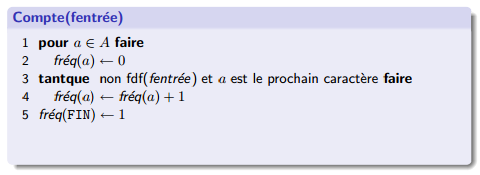
\includegraphics{comptage.PNG}
\end{center}
\item \textbf{Construction du code préfixe} : Un code préfixe est un ensemble de mots tel qu’aucun mot de
l’ensemble n’est préfixe d’un autre mot de l’ensemble. Un code préfixe sur l’alphabet binaire \{0, 1\} peut être représenté par
un tri qui est un fait un arbre binaire dont tous les nœuds internes ont exactement deux successeurs. Les feuilles sont étiquetées avec les caractères originaux, les branches par 0 ou 1 et les chemins depuis la racine jusqu’aux feuilles épellent les codes des caractères originaux. L’utilisation d’un code préfixe assure que les codes sont bien représentés par les feuilles. Par convention, le fils gauche d’un nœud est étiqueté par 0 et le fils droit
par 1.
\begin{center}
    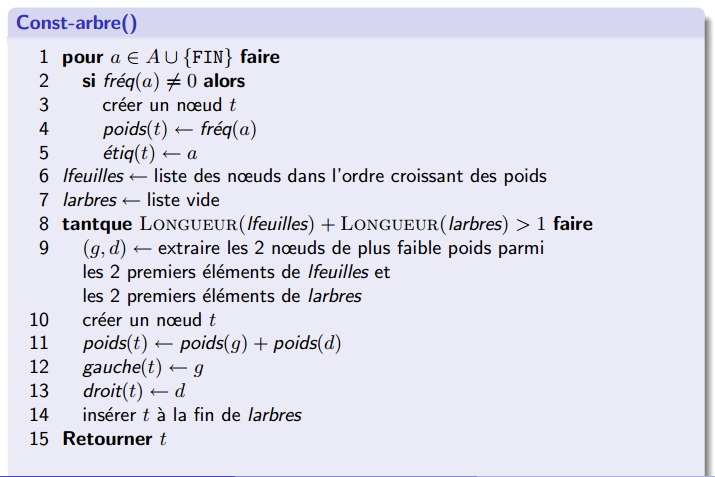
\includegraphics[scale=0.65]{arbre.PNG}
\end{center}
\item \textbf{Codage du texte} : Après la construction de l’arbre, il est possible de retrouver le code de
chaque caractère par un parcours en profondeur de l’arbre. 
\begin{center}
    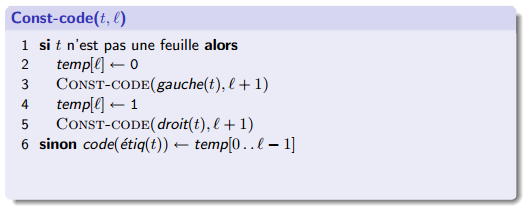
\includegraphics[scale=0.90]{constcode.PNG}
\end{center}
Cette étape nécessite de stocker les codes de chaque caractère avant le code du texte.
\begin{center}
    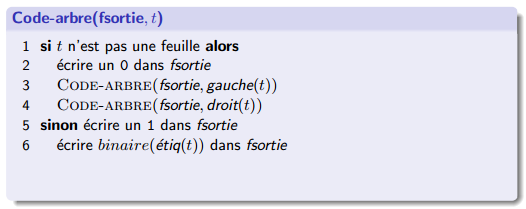
\includegraphics[scale=0.90]{codearbre.PNG}
\end{center}
On peut ensuite coder le texte.
\begin{center}
    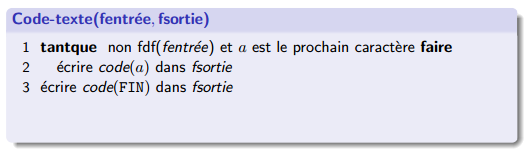
\includegraphics[scale=0.90]{codetexte.PNG}
\end{center}
La complexité de cette étape est le la complexité d'un parcours d'un arbre binaire, c'est-à-dire en $O(n log(n))$.\\
\end{enumerate}

\item \textit{Quelles sont les différentes étapes d'un algorithme de décompression de texte qui prend en entrée une version comprimée d'un texte à l'aide d'un codage de Huffman et fournit en sortie le texte original ? Soyez précis dans votre description en isolant chaque étape du problème. Précisez notamment pour chaque étape les structures de données utiles et la complexité temporelle des opérations menées.} (Alexis)\\

\item \textbf{[Question liée spécifiquement au problème posé]} En quoi les deux classes qui
vous sont fournies, \texttt{\textbf{InputBitStream}} et \texttt{\textbf{OutputBitStream}}, peuvent-elles
être utiles pour le problème de compression et de décompression avec un codage
de Huffman ? La postcondition de la méthode \texttt{\textit{close}} dans la classe \texttt{\textbf{OutputBitStream}}
précise notamment que \textit{si le nombre de bits déjà écrits ne correspond pas à un
multiple de 8 (un octet), des bits à 0 sont écrits pour compléter l’octet courant}.
Quand la situation décrite peut-elle se présenter ? Quelle est la conséquence de
cette postcondition sur votre programme de compression de texte ? Quelle est la
conséquence de cette postcondition sur votre programme de décompression ? \\(Xavier)\\
Les classes \texttt{\textbf{InputBitStream}} et \texttt{\textbf{OutputBitStream}} ont pour but de lire et d'écrire des bits, dont l'entrée et la sortie standard sont orientés vers les flux de caractères encodés en Unicode. La valeur d'un $int$ sur la sortie standard est une séquence de caractères (représentation décimale), tandis que la valeur d'un $int$ sur \texttt{\textbf{OutputBitStream}} est une séquence de bits (représentation binaire). Ces classes  fondent leur I/O sur 8-bit bytestreams. Les données sur l'entrée standard ne sont pas nécessairement alignés sur les frontières d'octets. La méthode \texttt{\textit{close}} n'est pas indispensable mais, pour une terminaison propre, les utilisateurs devraient appeler \texttt{\textit{close}} pour indiquer qu'il n'y a plus de bits à lire (pour la compression). Pour la décompression, la méthode \texttt{\textit{close}} est essentielle. En effet, les utilisateurs doivent appeler \texttt{\textit{close}} pour veiller à ce que tous les bits spécifiés avec les appels \texttt{\textit{write}} s'écrivent dans la $bitstream$ et que le dernier octet se remplisse avec des 0 afin que output s'aligne avec le système de fichiers.
\item \textbf{[Question liée spécifiquement au problème posé]} \textit{Donnez un diagramme détaillé des différentes classes et interfaces utilisées pour résoudre le problème de compression et de décompression de données. Précisez dans ce diagramme, les liens du type uses, implements ou extends. Quelles sont les classes qui sont communes entre les programmes de compression et de décompression de données ?}\\
Les classes compress et decompress utilisent respectivement InputStream et OutputStream pour leur bon fonctionnement. 
\begin{figure} [!h]
\center
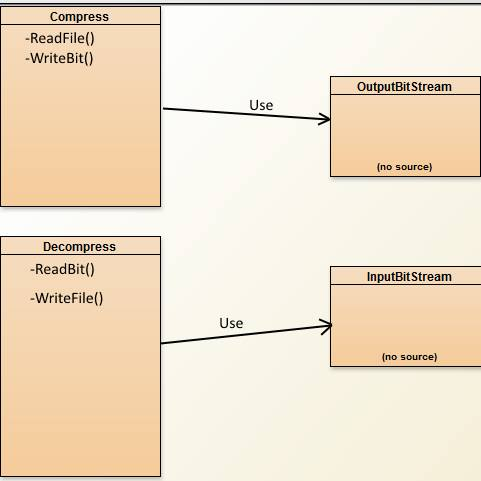
\includegraphics[scale=0.7]{diag.jpg}
\end{figure}
\item \textbf{[Question liée spécifiquement au problème posé]} \textit{Quel est le taux de compression
observé sur différents fichiers de texte ? Ce taux de compression dépend-il
de la taille du fichier ? Y a-t-il d’autres paramètres qui influencent ce taux de
compression ? Décrivez précisément les différents essais que vous aurez effectués
avec vos programmes de compression et de décompression de texte.
Quel est le temps de réponse moyen de votre programme de compression en
fonction de la taille du fichier de texte ? Quel est le temps de réponse moyen de
votre programme de décompression en fonction de la taille du fichier comprimé ?}
\textit{\textbf{Les temps calcul observés sont-ils cohérents avec la complexité temporelle
des algorithmes de compression/décompression ? Argumentez.}}

Cette question nécessite que notre implémentation du problème soit faite. 
Elle sera donc faite avec la deuxième partie du projet.

\end{enumerate}
\end{document}
